\documentclass[a4paper]{article}

\usepackage[style=ieee,backend=biber]{biblatex}
\usepackage{INTERSPEECH_v2}
\usepackage{lipsum} % we can remove this at the end
\renewcommand*\bibfont{\eightpt}

\addbibresource{references.bib}

\title{Paper Template for INTERSPEECH}
\name{Author Name$^1$, Co-author Name$^2$}
\address{
  $^1$Author Affiliation, Sweden\\
  $^2$Co-author Affiliation, Australia}
\email{author@university.edu, coauthor@company.com}

\begin{document}

\maketitle
% 
\begin{abstract}
% Copyright (C) 2016  Arvid Fahlström Myrman
%
% This program is free software; you can redistribute it and/or modify
% it under the terms of the GNU General Public License as published by
% the Free Software Foundation; either version 2 of the License, or
% (at your option) any later version.
%
% This program is distributed in the hope that it will be useful,
% but WITHOUT ANY WARRANTY; without even the implied warranty of
% MERCHANTABILITY or FITNESS FOR A PARTICULAR PURPOSE.  See the
% GNU General Public License for more details.
%
% You should have received a copy of the GNU General Public License along
% with this program; if not, write to the Free Software Foundation, Inc.,
% 51 Franklin Street, Fifth Floor, Boston, MA 02110-1301 USA.

\begin{abstract}
Unsupervised learning of speech is concerned with automatically finding patterns such as words or speech sounds, without supervision in the form of orthographical transcriptions or a priori knowledge of the language.
However, a fundamental problem is that unsupervised speech learning methods tend to discover highly speaker-specific and context-dependent representations of speech.
We propose a method for improving the quality of posteriorgrams generated from an unsupervised model through partitioning of the latent classes discovered by the model.
We do this by training a sparse siamese model to find a linear transformation of input posteriorgrams, extracted from the unsupervised model, to lower-dimensional posteriorgrams.
The siamese model makes use of same-category and different-category speech fragment pairs obtained through unsupervised term discovery.
After training, the model is converted into an exact partitioning of the posteriorgrams.
We evaluate the model on the minimal-pair ABX task in the context of the Zero Resource Speech Challenge.
We are able to demonstrate that our method significantly reduces the dimensionality of standard Gaussian mixture model posteriorgrams, while also making them more speaker invariant.
This suggests that the model may be viable as a general post-processing step to improve probabilistic acoustic features obtained by unsupervised learning.
\end{abstract}

\clearpage

\begin{otherlanguage}{swedish}
  \begin{abstract}
    Obevakad inlärning av tal innebär att automatiskt hitta mönster i tal, t~ex ord eller talljud, utan bevakning i form av ortografiska transkriptioner eller tidigare kunskap om språket.
    Ett grundläggande problem är dock att obevakad talinlärning tenderar att hitta väldigt talar- och kontextspecifika representationer av tal.
    Vi föreslår en metod för att förbättra kvaliteten av posteriorgram genererade med en obevakad modell, genom att partitionera de latenta klasserna funna av modellen.
    Vi gör detta genom att träna en gles siamesisk modell för att hitta en linjär transformering av de givna posteriorgrammen, extraherade från den obevakade modellen, till lågdimensionella posteriorgram.
    Den siamesiska modellen använder sig av talfragmentpar funna med obevakad ordupptäckning, där varje par består av fragment som antingen tillhör samma eller olika klasser.
    Den färdigtränade modellen görs sedan om till en exakt partitionering av posteriorgrammen.
    Vi följer Zero Resource Speech Challenge, och evaluerar modellen med hjälp av minimala ordpar-ABX-uppgiften.
    Vi demonstrerar att vår metod avsevärt minskar posteriorgrammens dimensionalitet, samtidigt som posteriorgrammen blir mer talarinvarianta.
    Detta antyder att modellen kan vara användbar som ett generellt extra steg för att förbättra probabilistiska akustiska särdrag från obevakade modeller.
  \end{abstract}
\end{otherlanguage}

\cleardoublepage

\end{abstract}
% check these
\noindent\textbf{Index Terms}: zero-resource speech challenge, unsupervised learning, speech recognition

% Copyright (C) 2016  Arvid Fahlström Myrman
%
% This program is free software; you can redistribute it and/or modify
% it under the terms of the GNU General Public License as published by
% the Free Software Foundation; either version 2 of the License, or
% (at your option) any later version.
%
% This program is distributed in the hope that it will be useful,
% but WITHOUT ANY WARRANTY; without even the implied warranty of
% MERCHANTABILITY or FITNESS FOR A PARTICULAR PURPOSE.  See the
% GNU General Public License for more details.
%
% You should have received a copy of the GNU General Public License along
% with this program; if not, write to the Free Software Foundation, Inc.,
% 51 Franklin Street, Fifth Floor, Boston, MA 02110-1301 USA.

% \begin{figure}
%   \centering
%   Sound + transcription + posteriorgrams
% 
%   \caption{\label{fig:postspec}Posteriorgram spectrum}
% \end{figure}

\chapter{Introduction}
\section{Background}
Automatic speech recognition (ASR) is generally framed as a supervised task, where both acoustic speech data and the corresponding transcription is available, and the problem is to develop a model that can mimic this mapping from speech to text.
However, developing such data is expensive, both in terms of time and money, as it involves painstakingly transcribing many hours of speech.
As a result, there is a notable lack of high-quality data for speech recognition for a majority of languages around the world.
An important question is thus whether it is possible to make use of untranscribed, or unlabelled, data to develop ASR for such low-resource languages.
Unsupervised learning in this manner may also provide insight into the linguistic structure of languages, or the language acquisition of infants.

In this work we focus in particular on one aspect of unsupervised learning of speech, namely the discovery of phonetic classes, i.e.\ the basic speech sounds that make up all words in a language.
While supervised speech recognition makes use of prior knowledge regarding what sounds are present in a language, in unsupervised acquisition of speech this knowledge is unavailable to us.
This means that not only do we need to be able to discover what sounds make up each word in a recording without the use of a transcription---we need to discover what sounds are even available in the language to begin with, as not all languages use the same sounds, nor are the same sounds contrastive in all languages.
This is compounded by speaker variation, where there can be significant differences between the pronunciation of sounds by individual speakers, or even by the same speaker depending on e.g.\ the context of the sound.
This variation makes approaches such as naive clustering ineffective, as many of the discovered sounds are likely to be highly speaker-specific.

Unsupervised speech acquisition is an area of active research.
One source of such research is the Zero Resource Speech Challenge \parencite{versteegh2015zero}, which was developed with the goal of finding linguistic units (track 1) or longer recurring word-like fragments (track 2) in speech.
Models are to be trained using only speech data, voice activity information, and speaker identity information.
The main goal of the first track of the challenge is to find robust representations of speech frames where sounds belonging to the same phonetic category are more similar than sounds belonging to different categories; this is also the approach we will take in this work.

% Copyright (C) 2016  Arvid Fahlström Myrman
%
% This program is free software; you can redistribute it and/or modify
% it under the terms of the GNU General Public License as published by
% the Free Software Foundation; either version 2 of the License, or
% (at your option) any later version.
%
% This program is distributed in the hope that it will be useful,
% but WITHOUT ANY WARRANTY; without even the implied warranty of
% MERCHANTABILITY or FITNESS FOR A PARTICULAR PURPOSE.  See the
% GNU General Public License for more details.
%
% You should have received a copy of the GNU General Public License along
% with this program; if not, write to the Free Software Foundation, Inc.,
% 51 Franklin Street, Fifth Floor, Boston, MA 02110-1301 USA.

\section{Related work}
\label{ch:related-work}

This \namecref{ch:related-work} provides a brief overview of recent research on unsupervised acoustic modelling.
The approaches discussed here can broadly be divided into two categories: frame-based approaches that infer the acoustic model directly from the speech frames, and term discovery-based approaches that first segment the speech into syllable- or word-like fragments, and afterwards try break these fragments into smaller subword units.
See \cref{ch:theory} for a more detailed description of some of the concepts mentioned here.

\subsection{Frame-based approaches}

While on an abstract level words and sentences are composed of a sequence of discrete speech sounds, on an acoustic level speech is a continuous signal, with smooth transitions between sounds.
In order to more easily analyse speech we therefore generally segment the speech signal into a sequence of short frames of equal size.

As an individual speech frame only makes up a fraction of a complete speech sound, it is natural to model the speech using a model that can capture time dependencies, such as a hidden Markov model (HMM), rather than attempt to cluster the speech frames directly.
One issue with this approach, however, is that the number of possible states (i.e.\ subword units) is unknown a priori.

\textcite{varadarajan2008unsupervised} tackle this problem by first defining a one-state HMM, and then iteratively splitting and merging states as needed to account for the data according to a heuristic.
Training stops once the size of the HMM reaches a threshold.
After training, each state in the HMM can be thought to correspond to some allophone (context-dependent variant realisation) of a phoneme.
It should be noted, however, that in order to interpret a given state sequence as a single phoneme, \citeauthor{varadarajan2008unsupervised} train a separate model using labelled speech to perform this mapping.
The method is thus not fully unsupervised.

\textcite{lee2012nonparametric} take a fully probabilistic approach, defining a model that jointly performs segmentation and acoustic modelling.
An infinite mixture model of three-state hidden Markov model-Gaussian mixture models (HMM-GMMs) modelling subword units is defined using the Dirichlet process, and latent variables representing segment boundaries are introduced.
The data can be thought to be generated by repeatedly sampling an HMM to model a segment, sampling a path through the HMM, and for each state in the path sampling a feature vector from the corresponding GMM.
The probability of transitioning from one unit to another is thus not modelled.
Inference of the model is done using Gibbs sampling.

\textcite{siu2014unsupervised} use an HMM of a more classic form to model the data.
An initial transcription of the data in terms of state labels is first generated in an unsupervised manner using a segmental GMM (SGMM).
The HMM is then trained by iteratively updating the parameters of the model keeping the transcription fixed, and estimating the most likely transcription keeping the parameters fixed.
Note that the number of allowed states are here defined in advance.
$n$-gram statistics are then collected from the transcription and used for tasks such as unsupervised keyword discovery.

Diverging from previous approaches using temporal models, \textcite{chen2015parallel} perform standard clustering of speech frames using an infinite Gaussian mixture model.
After training, the speech frames are represented as posteriorgrams, which have been shown to be more speaker invariant than other features such as mel frequency cepstral coefficients \parencite{zhang2010towards}.
Despite the simple approach, this turned out to be the overall best-performing model in the first track of the 2015 Zero Resource Speech Challenge \parencite{versteegh2016zero}.
\textcite{heck2016unsupervised} later further improved on the model by performing clustering in two stages, with an intermediate supervised dimensionality reduction step using the clusters derived from the first clustering step as target classes.

\textcite{synnaeve2016temporal} use a siamese network to create an embedding where speech frames close to each other are considered to belong to the same subword unit, while distant speech frames are said to differ.
A siamese network is a feedforward neural network that takes two inputs and adjusts its parameters to either maximise or minimise the similarity of the corresponding outputs \parencite{bromley1994signature}.

\subsection{Term discovery-based approaches}

An alternative to the frame-based approach is to first find longer pairs of word-like fragments using unsupervised term discovery (UTD).
These pairs can serve as constraints, since if both fragments in a pair correspond to the same word, then logically the sounds that make up the fragment pairs should be the same as well.
The rationale is that while at the frame level the same speech sound can seem quite different between different speakers or even different realisations of the sound by the same speaker, patterns over a longer duration of time are easier to identify; this idea is illustrated in \textcite{jansen2013weak}.

The methods discussed here generally use UTD systems based on the segmental dynamic time warping (S-DTW) developed by \textcite{park2008unsupervised}.
S-DTW works by repeatedly performing dynamic time warping (DTW) on two audio streams while constraining the maximum amount of warping allowed, each time changing the starting point of the DTW in both streams.
This yields a set of alignments, from which the stretches of lowest average dissimilarity in each alignment can be extracted.
Unfortunately, this approach is inherently $O(n^2)$ in time.
To remedy this, \textcite{jansen2011efficient} introduced an approximate version that uses binary approximations of the feature vectors to perform the calculations in $O(n \log n)$ time using sparse similarity matrices; this system also serves as the baseline for the second track of the Zero Resource Speech Challenge \parencite{versteegh2015zero}.

\textcite{jansen2011towards} describe a method for finding subword units by clustering HMM states.
The method assumes the availability of clusters corresponding to words, where each cluster contains multiple examples of the word in question in the form of audio.
For each word, an HMM is trained on all the corresponding examples, the number of states in the model being set to a number proportional to the average duration of the word.
The states from each HMM are then collected and clustered based on the similarity of their distributions, forming clusters that hopefully correspond to subword units.

\textcite{jansen2013weak} take somewhat of an inverse approach, starting by clustering the whole data on a frame level, with the assumption that each cluster will tend to correspond to some speaker- or context-dependent subword unit.
They then look at pairs of word-like fragments known to be of the same type and calculate how often clusters tend to co-occurr.
The clusters are then partitioned so that clusters that co-occurr often are placed in the same partition.

\textcite{synnaeve2014phonetics} introduce a neural network referred to as the ABnet, based on siamese networks \parencite{bromley1994signature}.
The network takes a pair of speech frames as input, and adjusts its parameters so that the outputs are collinear if the inputs are known to correspond to the same subword unit, and orthogonal otherwise, using a cosine-based loss function.
\textcite{thiolliere2015hybrid} made use of this approach in the Zero Resource Speech Challenge, also incorporating unsupervised term discovery so as to make the whole process unsupervised, yielding competitive results \parencite{versteegh2016zero}.
\textcite{zeghidour2016deep} experiment with supplying the ABnet with scattering spectrum features instead of filter bank features, showing that with the right features, a shallow architecture may outperform a deep architecture, especially when the amount of available data is low.

\textcite{kamper2015unsupervised} use an autoencoder-like structure, where a neural network is trained to ``reconstruct'' a frame given another frame known to be of the same type.
\textcite{renshaw2015comparison} used this architecture in the Zero Resource Speech Challenge, albeit with a deeper decoder.


\section{This thesis}

\begin{figure}
  \centering
  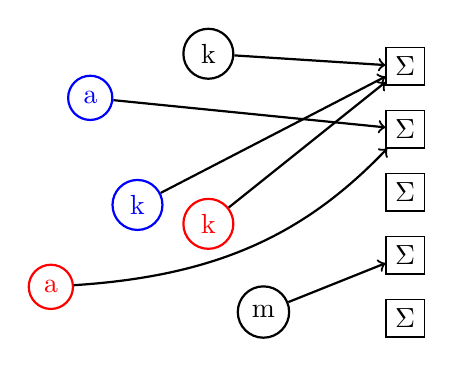
\begin{tikzpicture}[outpos/.style={draw,rectangle},inpos/.style={draw,circle,thick},
    arr/.style={->,thick},yscale=0.8]
    \node[outpos] at (0,0) {$\Sigma$};
    \node[outpos] (out3) at (0,1) {$\Sigma$};
    \node[outpos] at (0,2) {$\Sigma$};
    \node[outpos] (out2) at (0,3) {$\Sigma$};
    \node[outpos] (out1) at (0,4) {$\Sigma$};
    
    \node[inpos,blue] (a1) at (-4, 3.5) {a};
    \node[inpos,red] (a2) at (-4.5, 0.5) {a};
    \node[inpos,blue] (k1) at (-3.4, 1.8) {k};
    \node[inpos,red] (k2) at (-2.5, 1.5) {k};
    \node[inpos] (k3) at (-2.5, 4.2) {k};
    \node[inpos] (m1) at (-1.8, 0.1) {m};
    
    \draw (a1) edge[arr] (out2) (a2) edge[arr,bend right=24] (out2)
          (k1) edge[arr] (out1) (k2) edge[arr] (out1) (k3) edge[arr] (out1)
	  (m1) edge[arr] (out3);
  \end{tikzpicture}

  \caption{\label{fig:mapping}An example of merging speaker-specific (coloured) clusters by mapping them to (a subset of) the available outputs.
  As we represent the input as a probability vector, each output is a simple sum of the input probabilities.}
\end{figure}

We take inspiration from two of the most successful approaches so far: the GMM clustering approach of \textcite{chen2015parallel} and the siamese network approach of \textcite{thiolliere2015hybrid}, described above.
We pose the question of whether it is possible to combine the two approaches in order to take advantage of both the full unlabelled data set, as in the former approach, and the smaller set of discovered fragments, as in the latter approach.
One way to do this is to first cluster the whole data set in a fully unsupervised manner, discovering latent classes from the data such that similar data points belong to the same latent class.
After extracting a latent representation of the data from the clustering model, we can then improve on this representation using speech fragment information.

For this work we consider in particular probabilistic models such as Gaussian mixture models and hidden Markov models.
These models express class membership in terms of probabilities, giving the posterior probability of each data point belonging to one of the latent classes.
By representing each data point as a vector of these posterior probabilities, called a posteriorgram, the task of improving this representation can be framed as one of merging, or partitioning, the latent classes appropriately.
Latent classes discovered through unsupervised training will generally be highly speaker-specific.
However, by merging the classes using weak supervision in the form of speech fragment pairs, we can construct classes that are more speaker invariant.

A partitioning of classes can be viewed as finding a function which maps the original set of classes to a class set of lower cardinality, but finding this function is a discrete problem which is difficult to optimise for.
However, a benefit of posteriorgrams is that the probability of an output class can be described as a simple sum of the probabilities of the input classes that map to the output in question, as illustrated in \cref{fig:mapping}.
This means that the mapping function can be approximated using a continuous linear model which can be optimised through standard gradient descent.
A linear model also has the benefit of being more interpretable than deep networks such as that of \textcite{thiolliere2015hybrid}.
While the approach of partitioning posteriorgrams is very reminiscent of \textcite{jansen2013weak}, the major difference is that in place of direct clustering of classes, we are instead trying to maximise the similarity/dissimilarity between pairs of speech fragments, which only indirectly results in a partitioning of the classes.

\begin{figure}
  \centering
  \begin{tikzpicture}
    %\begin{axis}[enlargelimits=false,axis on top,width=8cm,height=4cm,ylabel={Frequency (\si\Hz)},xlabel={Time (\si\s)}]
    %\end{axis}

% speaker 1
% s3102b 146.518752 147.111647 questions
%   146.518752  122 ng
%   146.596735  122 k
%   146.624258  122 w
%   146.693066  122 ah
%   146.760727  122 s; *
%   146.816920  122 ch
%   147.021050  122 en
%   147.111647  122 z

% speaker 2
% s2302a 106.778375 107.628939 questions
%   106.778375  122 ng
%   106.883302  122 k
%   106.921215  122 w
%   106.985553  122 eh
%   107.098375  122 s ; *
%   107.168375  122 ch
%   107.246360  122 ah
%   107.348375  122 n
%   107.628939  122 z
    \begin{groupplot}[group style={group size=2 by 3, horizontal sep=1.3cm, vertical sep=0.4cm},
      enlargelimits=false,width=5cm,height=4.5cm,axis on top,xtick=\empty]
      \nextgroupplot[ylabel={Frequency (\si\Hz)},title={Female speaker}]
      \addplot graphics[xmin=146.52,xmax=147.11,ymin=0,ymax=3125] {data/spectrum-speaker-1-crop.pdf};
      \coordinate (kw1t) at (axis cs:146.59,\pgfkeysvalueof{/pgfplots/ymax});
      \coordinate (we1t) at (axis cs:146.62,\pgfkeysvalueof{/pgfplots/ymax});
      \coordinate (es1t) at (axis cs:146.69,\pgfkeysvalueof{/pgfplots/ymax});
      \coordinate (sc1t) at (axis cs:146.76,\pgfkeysvalueof{/pgfplots/ymax});
      \coordinate (cu1t) at (axis cs:146.82,\pgfkeysvalueof{/pgfplots/ymax});
      \coordinate (un1t) at (axis cs:147.02,\pgfkeysvalueof{/pgfplots/ymax});

      \nextgroupplot[title={Male speaker}]
      \addplot graphics[xmin=106.78,xmax=107.63,ymin=0,ymax=3125] {data/spectrum-speaker-2-crop.pdf};
      \coordinate (kw2t) at (axis cs:106.88,\pgfkeysvalueof{/pgfplots/ymax});
      \coordinate (we2t) at (axis cs:106.92,\pgfkeysvalueof{/pgfplots/ymax});
      \coordinate (es2t) at (axis cs:106.99,\pgfkeysvalueof{/pgfplots/ymax});
      \coordinate (sc2t) at (axis cs:107.10,\pgfkeysvalueof{/pgfplots/ymax});
      \coordinate (cu2t) at (axis cs:107.17,\pgfkeysvalueof{/pgfplots/ymax});
      \coordinate (un2t) at (axis cs:107.35,\pgfkeysvalueof{/pgfplots/ymax});
      
      \nextgroupplot[ylabel={GMM component}]
      \addplot graphics[xmin=146.52,xmax=147.11,ymin=1,ymax=1024] {data/gmm-posteriorgrams-speaker-1-crop.pdf};
      
      \nextgroupplot
      \addplot graphics[xmin=106.78,xmax=107.63,ymin=1,ymax=1024] {data/gmm-posteriorgrams-speaker-2-crop.pdf};
      
      \nextgroupplot[ylabel={Model output},xlabel={Time}]
      \addplot graphics[xmin=146.52,xmax=147.11,ymin=1,ymax=33] {data/reduced-posteriorgrams-speaker-1-crop.pdf};
      \coordinate (kw1b) at (axis cs:146.59,\pgfkeysvalueof{/pgfplots/ymin});
      \coordinate (we1b) at (axis cs:146.62,\pgfkeysvalueof{/pgfplots/ymin});
      \coordinate (es1b) at (axis cs:146.69,\pgfkeysvalueof{/pgfplots/ymin});
      \coordinate (sc1b) at (axis cs:146.76,\pgfkeysvalueof{/pgfplots/ymin});
      \coordinate (cu1b) at (axis cs:146.82,\pgfkeysvalueof{/pgfplots/ymin});
      \coordinate (un1b) at (axis cs:147.02,\pgfkeysvalueof{/pgfplots/ymin});
      
      \nextgroupplot[xlabel={Time}]
      \addplot graphics[xmin=106.78,xmax=107.63,ymin=1,ymax=33] {data/reduced-posteriorgrams-speaker-2-crop.pdf};
      \coordinate (kw2b) at (axis cs:106.88,\pgfkeysvalueof{/pgfplots/ymin});
      \coordinate (we2b) at (axis cs:106.92,\pgfkeysvalueof{/pgfplots/ymin});
      \coordinate (es2b) at (axis cs:106.99,\pgfkeysvalueof{/pgfplots/ymin});
      \coordinate (sc2b) at (axis cs:107.10,\pgfkeysvalueof{/pgfplots/ymin});
      \coordinate (cu2b) at (axis cs:107.17,\pgfkeysvalueof{/pgfplots/ymin});
      \coordinate (un2b) at (axis cs:107.35,\pgfkeysvalueof{/pgfplots/ymin});

  \end{groupplot}
  \draw [thin,white] (kw1t) -- (kw1b);
  \draw [thin,white] (we1t) -- (we1b);
  \draw [thin,white] (es1t) -- (es1b);
  \draw [thin,white] (sc1t) -- (sc1b);
  \draw [thin,white] (cu1t) -- (cu1b);
  \draw [thin,white] (un1t) -- (un1b);
  
  \draw [thin,white] (kw2t) -- (kw2b);
  \draw [thin,white] (we2t) -- (we2b);
  \draw [thin,white] (es2t) -- (es2b);
  \draw [thin,white] (sc2t) -- (sc2b);
  \draw [thin,white] (cu2t) -- (cu2b);
  \draw [thin,white] (un2t) -- (un2b);
  \end{tikzpicture}

  \caption{\label{fig:model-output}Example of using the proposed model to process utterances of the word ``question'' from two different speakers.
  First the energy spectrum is calculated for each speech frame (top).
  After preprocessing the spectrum is then fed to a Gaussian mixture model from which posterior probabilities for each latent class is extracted (middle).
  Last, the probability vectors from the GMM are reduced in size using the proposed model (bottom).
  The white crosses mark the most probable class state for each frame.
  The white vertical lines mark boundaries between speech sounds.
  The example is meant to be illustrative and does not represent the overall performance of the model.}
\end{figure}

Using such a linear model, we hope to use speech fragment information to improve on posteriorgrams obtained from an unsupervised probabilistic model.
In particular we hope to use the model to construct more speaker-invariant posteriorgrams which can be used to discriminate between different linguistic units in a robust manner.
An example of using the model can be seen in \cref{fig:model-output}; the model takes high-dimensional posteriorgrams describing a probability distribution over latent variables (classes) from a Gaussian mixture model, and outputs low-dimensional posteriorgrams which are more speaker invariant.
We evaluate the model using the minimal-pair ABX task used for evaluation in the first track of the Zero Resource Speech Challenge.
The minimal-pair ABX task aims to evaluate the quality of different representations of speech by ensuring that two utterances of the same word are more similar to each other than to a distinct but similar word.

\section{Method}
\label{sec:method}
% Arvid: check that I am not getting this wrong
The goal of our method is to merge acoustic clusters obtained by bottom-up unsupervised classification such that the resulting classes correspond more closely to phonemic units in the language.


We take as input a set $\{(\mat x_i, \mat y_i)\}_{i=1}^N$ of $N$ pairs of $M$-dimensional posteriorgrams, i.e.\ (row) vectors of probabilities such that the probabilities sum to one.
Additionally, we have a set of indicators $\{c_i\}_{i=1}^N$ such that $c_i$ is $1$ if $\mat x_i$ and $\mat y_i$ belong to the same class, and $0$ otherwise.
The posteriorgrams are taken to represent a distribution over $M$ discrete ``pseudo''-classes (e.g.\ allophones), where several pseudo-classes together describe a single ``true'' class (e.g.\ phonemes).
Our goal is then to find a surjection that maps the $M$ pseudo-classes to a smaller set of $D$ classes, where we take the probability of a single output class to be the sum of the probabilities of the pseudo-classes that map to the class in question.

To simplify optimisation we relax the problem to one of instead finding a continuous linear mapping $f : [0,1]^M \to [0,1]^D$ from the original space to a lower-dimensional space, such that $f(\mat x_i)$ and $f(\mat y_i)$ are close if $\mat x_i$ and $\mat y_i$ belong to the same true class, and distant otherwise.
We consider each output probability to be a weighted combination of input probabilities: $f(\mat x)_j = \sum_{i=1}^M x_i w_{ij}$, or in matrix notation:
\begin{equation}
 f(\mat x) = \mat x \mat W
\end{equation}
where $\mat W = (w_{ij}) \in \mathbb R^{M \times D}$.
If the elements of $\mat W$ are constrained to only take on values in $\{0, 1\}$, and each row of $\mat W$ contains exactly one element with the value $1$, the problem is reduced to finding an exact surjection.

Even in the relaxed version of the problem, we need to put certain constraints on $\mat W$ in order to ensure that the output $f(\mat x)$ is a posteriorgram.
First, we need to ensure that all outputs are positive.
As the input $\mat x$ is a posteriorgram, meaning that all elements in $\mat x$ are positive, it clearly suffices to ensure that all elements in $\mat W$ are positive.
Second, the output probabilities must sum to 1.
This can be achieved by ensuring that the elements of each row of $\mat W$ sum to 1, as can be seen by:
\begin{equation}
 f(\mat x) \mat 1_D = \mat x \mat W \mat 1_D = \mat x \mat 1_D = 1
\end{equation}
where $\mat 1_D$ is a column vector of $D$ ones.

In order to ensure that these constraints hold, we construct our model as follows:
\begin{align}
  \mat V &\in \mathbb R^{M \times D} \\
  \mat{\widetilde W} &= |\mat V| \\
  \mat W &= \mat{\widetilde W} \oslash \left(\mat{\widetilde W} \mat 1_D \mat 1_D^T\right) \\
  f(\mat x) &= \mat x \mat W
\end{align}
where $|\cdot|$ denotes the element-wise absolute value, and $\oslash$ denotes element-wise division.
This formulation makes it possible to optimise the model while ensuring that the constraints on $\mat W$ hold, by performing gradient descent with respect to $\mat V$.
Note that the absolute value is almost everywhere differentiable, and the non-differentiability at $0$ does not matter in practice.

To encourage the model to place points belonging to the same class close together in the output space, we consider the model as a siamese network.
Conceptually this involves duplicating the model, creating two identical copies of the same network, with the parameters shared.
We then feed one input each to both copies, and calculate the loss function using the corresponding outputs:
\begin{equation}
  L(\mat V; \mat x, \mat y, c) = \begin{cases}D_{\mathrm{same}}(f(\mat x; \mat V), f(\mat y; \mat V)) & \text{if } c = 1 \\
    D_{\mathrm{diff}}(f(\mat x; \mat V), f(\mat y; \mat V)) & \text{if } c = 0\end{cases}
\end{equation}
where $D_{\mathrm{same}}$ and $D_{\mathrm{diff}}$ are the dissimilarity/similarity measures for pairs belonging to the same class, and pairs belonging to different classes, respectively.
The loss function over a minibatch $B$ is given by the average
\begin{equation}
  \frac{1}{|B|} \sum_{i \in B} L(\mat V; \mat x_i, \mat y_i, c_i)
\end{equation}
which is minimised with respect to $\mat V$.

\subsection{Loss function}

As the output of the model is a probability distribution, it makes intuitive sense to use a statistical divergence as a measure of similarity.
Perhaps the most well-known divergence is the Kullback-Leibler (KL) divergence, defined as:
\begin{equation}
  \mathrm{KL}(\mat x || \mat y) = \sum_i x_i \log_2\frac{x_i}{y_i},
\end{equation}
where we take $0 \log_2 0$ to be $0$.
The KL divergence is always positive, and is 0 only if $\mat x = \mat y$.
However, it is unbounded, and undefined if there is an $i$ such that $y_i = 0$ but $x_i \ne 0$.
As such, trying to maximise the dissimilarity between two distributions with respect to the KL divergence is an ill-posed problem, as this will force the divergence to tend towards infinity.

A better choice is the Jensen-Shannon (JS) divergence, defined as
\begin{equation}
  \mathrm{JS}(\mat x || \mat y) = \frac{1}{2} \mathrm{KL}(\mat x || \mat m) + \frac{1}{2} \mathrm{KL}(\mat y || \mat m)
\end{equation}
where $\mat m = (\mat x + \mat y)/2$.
The JS divergence is always defined, and is bounded between $0$ (for identical distributions) and $1$ (for distributions with disjoint support), assuming that the base 2 logarithm is used.
Additionally, the square root of the JS divergence is a metric satisfying the triangle inequality \parencite{endres2003new}; here we make use of this fact, in the hope that the metric properties will result in a more well-behaved loss function.

Thus, we define the loss function as
\begin{equation} \label{eq:js-loss}
  L_{\mathrm{JS}}(\mat V; \mat x, \mat y, c) = \begin{cases}
    \sqrt{\mathrm{JS}(f(\mat x; \mat V) || f(\mat y; \mat V))} & \text{if } c = 1 \\
    1 - \sqrt{\mathrm{JS}(f(\mat x; \mat V) || f(\mat y; \mat V))} & \text{if } c = 0,
  \end{cases}
\end{equation}
thereby minimising the root JS divergence between pairs belonging to the same class, and maximising the divergence between pairs belonging to different classes\footnote{For identical or near-identical $\mat x$ and $\mat y$, the JS divergence may become negative due to rounding errors caused by limited floating point precision; this can be counteracted by adding a small constant value before taking the square root.}.

\subsection{Entropy penalty}

To make the output of the model interpretable, it is desirable to ensure that for a given input, only one output unit is active.
This can be done by introducing an entropy penalty, which attempts to minimise the spread of the probability mass.
The entropy of a probability vector $\mat x = (x_1, \dots, x_D)$ is defined as
\begin{equation}
  H(\mat x) = -\sum_{i=1}^D x_i \log_2 x_i.
\end{equation}
However, this definition is sensitive to the value of $D$; for instance, the entropy of a uniform distribution vector is $\log_2 D$.

As we may wish to vary the number of outputs of the model, it is of interest for the entropy penalty to be invariant to the number of outputs.
We therefore introduce the normalised entropy, defined as
\begin{equation}
  \hat H(\mat x) = \frac{1}{\log_2 D} H(\mat x).
\end{equation}
The normalised entropy is always between 0 (for degenerate distributions) and 1 (for uniform distributions).

The entropy penalty implicitly encourages sparsity in $\mat W$, as the only way to avoid spreading the probability mass across several outputs is for each row of $\mat W$ to only contain a single element close to $1$.
It is thus through this penalty that we enforce the model to find an approximate surjection.
In summary, our final loss function over a minibatch $B$ is as follows:
\begin{multline}
  \label{eq:original-loss}
  L(\mat V; B) = \frac{1}{|B|} \sum_{i \in B} L_{\mathrm{JS}}(\mat V; \mat x_i, \mat y_i, c_i) + \\ 
  +\frac{\lambda}{2|B|} \sum_{i \in B} \left(\hat H\left(f(\mat x_i; \mat V)\right) + \hat H\left(f(\mat y_i; \mat V)\right)\right)
\end{multline}
where $\lambda$ is a hyperparameter.


%%% Local Variables: 
%%% enable-local-variables: t
%%% ispell-local-dictionary: "british"
%%% mode: latex
%%% eval: (flyspell-mode)
%%% eval: (flyspell-buffer)
%%% End: 

\section{Experiments}
\label{sec:experiments}

\subsection{Data}
To test our method we use the data from the 2015 Zero Resource Speech Challenge.
The Challenge makes use of two corpora: The Buckeye corpus of conersational English \parencite{buckeyecorpus} and the NCHLT speech corpus of read Xitsonga \parencite{barnard2014nchlt}.
For the challenge only a subset of the data is used, consisting of 12 speakers for a total of 5 hours of data for the Buckeye corpus, and 24 speakers for a total of 2.5 hours of data for the NCHLT Xitsonga corpus.
Additionally provided is voice activity information indicating segments containing clean speech, as well as labels indicating the identity of the speaker.

MFCCs features were extracted from the data using a frame window length \SI{25}{\ms} which was shifted \SI{10}{\ms} for each frame, an FFT resolution of 512 frequency steps, and 40 mel-spaced triangular filter banks.
13 coefficients with both delta and delta-delta features were used.
The MFCCs corresponding to segments with voice activity were clustered using an implementation of a Gaussian mixture model (GMM) provided by scikit-learn \parencite{scikit-learn}.
The GMM was trained using the expectation maximisation algorithm, using $M = 1024$ Gaussians with diagonal covariance matrices, for a maximum of 200 iterations.
After training posteriorgrams are calculated for each frame.

The unsupervised term discovery yielded 6512 fragments and 3149 clusters for the Buckeye corpus, and 3582 fragments and 1782 clusters for the NCHLT Xitsonga corpus\footnote{The cluster files used for this work were generously provided by Roland Thiollière and Aren Jansen.}.
70\% of the same-class and different-class fragment pairs were used for training, with the remaining pairs used for validation to determine when to interrupt the training of the models.

%\subsection{Unsupervised term discovery}
%\label{sec:utd}

% Pairs of similar speech fragments were discovered using the system developed by \textcite{jansen2011efficient}, which serves as a baseline for the second track of the Zero Resource Speech Challenge.
% The system works by calculating the approximate cosine similarity between pairs of frames of two input audio segments, based on discretised random projections of PLP features.
% For efficiency only frames found using an approximate nearest neighbour search are compared, yielding a sparse similarity matrix.
% Stretches of similar frames are then found by searching for diagonals in the similarity matrix, which which are then aligned using dynamic time warping (DTW).
% Pairs of segments with a DTW score above a certain threshold are kept and clustered based on pairwise DTW similarity, resulting in a set of clusters of speech segments, or fragments, thought to be of the same class (e.g.\ word).

% For each cluster every possible pair of fragments was extracted from the collection of posteriorgrams retrieved from the GMM and aligned using DTW, yielding pairs of speech frames belonging to the same class.
% Let $K$ be the total number of pairs of fragments aligned.
% To generate a set of pairs of frames belonging to different classes, $K$ fragments were sampled uniformly from the full collection of fragments.
% For each such fragments, another fragment was sampled uniformly from the fragments belonging to a different cluster.
% When sampling fragments belonging to a different cluster, the sampling was performed using only either fragments spoken by the same speaker, or fragments spoken by a different speaker, with a probability corresponding to the ratio of same-speaker to different-speaker pairs among the same-class fragment pairs.
% The different-class fragment pairs were aligned by simply truncating the longer fragment.

\subsection{Model implementation}
\todo[inline]{mention server specification? cpu/ram/gpu}

We used $D = 64$ outputs for all models.
The models were trained using AdaMax \parencite{kingma2014adam} with the recommended default parameters $\alpha = 0.002$, $\beta_1 = 0.9$ and $\beta_2 = 0.999$.
All frames used for training were shuffled once at the start of training, and a minibatch size of 1000 frames was used.
The models were trained until no improvement had been observed on a held-out validation set for 15 epochs, where one epoch is defined as one complete scan over the training data.

All network models were implemented in Python 3.5 using Theano \parencite{theano} for automatic differentiation and GPU acceleration, librosa \parencite{librosa} for feature extraction, scikit-learn \parencite{scikit-learn} for various utilities, and numba \parencite{numba} for accelerating various code, in particular dynamic time warping.

\subsection{Tuning the entropy penalty}
The entropy penalty $\lambda$ is a free parameter, which is data dependent and must be manually specified.
Ideally, $\lambda$ should be such that the entropy is reduced to a satisfactory degree, without sacrificing the Jensen-Shannon loss.
As both the normalised entropy loss and the Jensen-Shannon loss are bounded between 0 and 1, one might expect the optimal value of $\lambda$ to be in the vicinity of $1$.
Section~\ref{sec:results} reports on the optimisation of $\lambda$ with respect to the validation error both for the Buckeye and NCHLT Xitsonga corpora.

\subsection{Balancing same-class and different-class losses}
When enforcing low entropy in the output distribution, the resulting weight matrix becomes sparse.
For instance, after training the model with $\lambda = 0.1$, and inspecting the row-normalised matrix $\mat W$, we find that the largest element on each row is close to 1: on average across the 1024 rows $0.98$ for English and $0.92$ for Xitsonga.
We can thus inspect $\mat W$ to see how many of the $64$ outputs are actually being used by the model.
We take the sum over each column of $\mat W$.
This sum describes roughly how many inputs are mapped to each output.
We find that for both English and Xitsonga, this sum is above $0.5$ for only a minority of outputs: 11 outputs for English, and 10 outputs for Xitsonga.
For English, where $\mat W$ is particularly sparse, none of the other 53 sums even reach $0.05$.

Thus, it seems that the entropy penalty naturally encourages the model to make use of only a subset of the outputs.
However, the actual number of outputs used is not realistic in terms of how many phonemes one would expect to find in a language; it seems that the same-class loss is forcing too many input classes to merge.
To solve this, we restate the Jensen-Shannon loss function, allowing us to specify how much relative weight to give to the same-class and different-class losses.
Let $B_1 = \{i \in B : c_i = 1\}$ be the subset of same-class frame pairs in the current minibatch, and $B_0 = \{i \in B : c_i = 0\}$ the subset of different-class frame pairs.
We then restate the loss as
\begin{equation}
  \label{eq:rebalanced}
  \frac{1}{(\alpha + 1)|B_1|} \sum_{i \in B_1} L_{\mathrm{same}}(\mat V; \mat x_i, \mat y_i) + \frac{\alpha}{(\alpha + 1)|B_0|} \sum_{i \in B_0} L_{\mathrm{diff}}(\mat V; \mat x_i, \mat y_i),
\end{equation}
where $L_{\mathrm{same}}$ and $L_{\mathrm{diff}}$ are the same-class and different-class losses defined in \cref{eq:js-loss}.
$\alpha$ is a hyperparameter specifying how much more to weight the different-class loss over the same-class loss.

$\alpha$ needs to be carefully tuned: A too small $\alpha$ will cause too many input classes to merge, including classes that correspond to completely different phonemes, while a too large $\alpha$ will cause input classes that do correspond to the same phoneme to fail to merge.
In order to find a good value for $\alpha$, without making use of the gold transcription or prior knowledge of the number of phonemes present in the languages in question, we make use of the fragment clusters discovered by the unsupervised term discovery system.
The intuition is that the goal of our model is to push apart different clusters, while keeping fragments within a cluster as similar as possible.
To measure the success of our model, then, we can make use of a cluster separation measure.

Here we use the silhouette \parencite{rousseeuw1987silhouettes}, which makes use of the average similarity between a sample and every other sample in the same cluster, and between a sample and every sample in the most similar other cluster.
The silhouette ranges from -1 to 1, with a value close to 1 indicating that the clusters are well separated.
Models were trained for $\alpha \in \{1, 1.5, 2, 2.5, 3, 3.5, 4\}$, with an entropy penalty of $\lambda = 0.1$.
The silhouette was then calculated on a subset of 1000 of the fragment clusters, using the output of the trained models to represent the frames of the fragments.
The similarity between to fragments was calculated as the DTW score using the symmetrise Kullback-Leibler divergence as a similarity measure between individual frames.

\todo[inline]{is the below paragraph uninteresting? a bit too model-specific?}
To easily get an estimate of the number of outputs used by the model, we also define the ``spread'' of the model as follows.
We take the average of the $j$th column:
\begin{equation}
  q_j = \frac{1}{M} \sum_{i=1}^M w_{ij}.
\end{equation}
This represents the average mapping to the $i$th output.
As $\mat W$ is row-normalised, the elements of $Q = (q_1, q_2, \dots, q_D)$ sum to 1, and we can thus treat $Q$ as describing a probability distribution.
A uniform distribution means that each output has the same number of inputs mapped to it.
Now consider the case where there are $K$ outputs such that the same number of inputs maps to each output, while no inputs map to any other outputs.
The normalised entropy of $Q$ is then given by
\begin{equation}
  \hat H(Q) = - \frac{1}{\log_2 D} \sum_{i=1}^K \frac{1}{K} \log_2 \frac{1}{K} = \frac{\log_2 K}{\log_2 D}.
\end{equation}
Solving for $K$ we have
\begin{equation}
  K = D^{\hat H(Q)},
\end{equation}
which is an approximation of the number of outputs used by the model, which we define as the spread.
A value of $K$ close to $D$ is an indicator that all the outputs are being used equally, suggesting that it may be a good idea to increase the number of outputs.

\begin{figure}
 \centering
 \begin{tikzpicture}
   \pgfplotsset{set layers}
   \begin{axis}[
     scale only axis,
     xmin=0.8,xmax=4.2,
     ymax=0.25,
     axis y line*=left,
     xlabel=$\alpha$,
     ylabel=Silhouette,
     ylabel near ticks,
     yticklabel style={/pgf/number format/fixed},
     height=0.6\columnwidth,width=0.8\columnwidth,
     legend style={opacity=0.0}]%,
      %legend style={column sep=10pt},legend entries={Silhouette (English),Silhouette (Xitsonga)},legend cell align=left]
      \addplot table[x=alpha,y=sil-en] {data/silhouette.txt}; \label{sil1}
      \addlegendentry{Silhouette (English)}
   %\addplot+[mark=x] table[x=alpha,y=spread-en] {data/silhouette.txt};
   \addplot table[x=alpha,y=sil-ts] {data/silhouette.txt}; \label{sil2}
   \addlegendentry{Silhouette (Xitsonga)}
   %\addplot+[mark=x] table[x=alpha,y=spread-ts] {data/silhouette.txt};
   \end{axis}
   \begin{axis}[
     scale only axis,
     xmin=0.8,xmax=4.2,
     ymax=80,
     axis y line*=right,
     axis x line=none,
     ylabel=Spread,
     ylabel near ticks,
     height=0.6\columnwidth,width=0.8\columnwidth,
     legend style={anchor=north west,at={(0.02,0.98)}}]%,
      %legend style={column sep=10pt},legend entries={Silhouette (English),Silhouette (Xitsonga)},legend cell align=left]
   %\addplot+[mark=x] table[x=alpha,y=sil-en] {data/silhouette.txt};
   \addlegendimage{/pgfplots/refstyle=sil1}\addlegendentry{Silhouette (English)}
   \addlegendimage{/pgfplots/refstyle=sil2}\addlegendentry{Silhouette (Xitsonga)}
   \addplot+[dashed] table[x=alpha,y=spread-en] {data/silhouette.txt};
   \addlegendentry{Spread (English)}
   %\addplot+[mark=x] table[x=alpha,y=sil-ts] {data/silhouette.txt};
   \addplot+[dashed] table[x=alpha,y=spread-ts] {data/silhouette.txt};
   \addlegendentry{Spread (Xitsonga)}
   \end{axis}
 \end{tikzpicture}

 \caption{\label{fig:silhouette} Silhouette and spread for different weightings of the same-class and different-class losses.}
\end{figure}

\Cref{fig:silhouette} shows the silhouette and spread for different values of $\alpha$.
As one might expect, more emphasis on the different-class loss results in a higher spread, i.e.\ a larger number of output classes.
The optimal value of $\alpha$ seems to be around 1.5 for both data sets, we use this value of $\alpha$ going forward.

\subsection{Discretising the model}
\label{sec:discrete}
As the resulting model is sparse, we can retrieve an exact surjection by discretising the model.
We do this by for each row in $\mat W$ setting the largest element to $1$ and the remaining elements to $0$.
Using the discretised model as a base, we additionally experiment with discretising the output distribution by setting the largest output to 1 and the rest to 0; this can be thought of as taking the argmax of the output distribution.

\subsection{Comparison with deep models}
\label{sec:deep}
To get an idea of how the JS loss performs in general, we build a deep network with two hidden layers of $500$ sigmoid units each, with $64$ softmax outputs.
The network is trained using the non-rebalanced JS loss.
As softmax outputs are naturally sparse, we do not enforce any entropy penalty.
For comparison we train the same architecture, albeit with sigmoid outputs instead, using the coscos$^2$ loss of \textcite{synnaeve2014phonetics}.
This is the architecture used by \textcite{thiolliere2015hybrid} in the 2015 Zero Resource Speech Challenge.

As input to both networks we use the log-scale outputs of 40 mel-scaled filter banks.
All other relevant parameters are the same as for the MFCCs calculated in \cref{sec:posteriorgrams}.
The filter bank outputs are normalised over the whole data set to have zero mean and unit variance for all dimensions.
Each frame is fed to the network with a context of 3 frames on both sides, for a total of 280 values used as input to the network.
All fragments are DTW aligned and sampled as in \cref{sec:utd}.

%%% Local Variables: 
%%% enable-local-variables: t
%%% ispell-local-dictionary: "british"
%%% mode: latex
%%% eval: (flyspell-mode)
%%% eval: (flyspell-buffer)
%%% End: 

\section{Results}
\label{sec:results}

\subsection{Tuning the entropy penalty}
We train models using $\lambda \in \{0, 0.05, 0.1, \dots, 0.95\}$ for both the Buckeye and NCHLT Xitsonga corpora.
The final validation errors for each model are reported in \cref{fig:entropy-penalty}.
For both corpora, the entropy drops quickly even for small $\lambda$, suggesting that the entropy is relatively easy to optimise for.
As the entropy penalty is increased, the entropy itself does not decrease; however, the different-class JS loss decreases at the expense of the same-class JS loss. \todo{why?}
For future experiments, a penalty of $\lambda = 0.1$ is used.

\begin{figure*}
  \centering
  \begin{tikzpicture}
    \begin{groupplot}[group style={group size=2 by 1, horizontal sep=2cm},xmin=0,xmax=1,ymin=0,ymax=1,width=5cm,height=4cm]
      \nextgroupplot[title=English,xlabel=Penalty ($\lambda$),ylabel=Divergence/entropy,
      legend style={column sep=10pt},legend entries={JS loss,Same-class loss,Different-class loss,Normalised entropy},
      legend columns=2,legend to name=grouplegend,legend cell align=left]
   \addplot table[x=lambda,y=js-v] {data/entropy_buckeye.txt};
   \addplot table[x=lambda,y=same-js-v] {data/entropy_buckeye.txt};
   \addplot table[x=lambda,y=diff-js-v] {data/entropy_buckeye.txt};
   \addplot table[x=lambda,y=entropy-v] {data/entropy_buckeye.txt};
   
   \nextgroupplot[title=Xitsonga,xlabel=Penalty ($\lambda$),ylabel=Divergence/entropy]
   \addplot table[x=lambda,y=js-v] {data/entropy_xitsonga.txt};
   \addplot table[x=lambda,y=same-js-v] {data/entropy_xitsonga.txt};
   \addplot table[x=lambda,y=diff-js-v] {data/entropy_xitsonga.txt};
   \addplot table[x=lambda,y=entropy-v] {data/entropy_xitsonga.txt};
  \end{groupplot}
  \node[yshift=1.6cm] at ($(group c1r1.north)!.5!(group c2r1.north)$) {\ref{grouplegend}};
\end{tikzpicture}

\caption{\label{fig:entropy-penalty} Effect of varying the entropy penalty for the English (left) and Xitsonga (right) corpora.
The average entropy of the output distribution over the validation samples is shown along with the (root) Jensen-Shannon loss: Both the combined JS loss that is optimised for, and separately for same-class and different-class frame pairs.}
\end{figure*}

\subsection{ABX evaluation}
\begin{table*}
 \centering
 \begin{tabular}{lrrrrrr} \toprule
   & \multicolumn{3}{c}{English} & \multicolumn{3}{c}{Xitsonga} \\ \cmidrule(lr){2-4} \cmidrule(lr){5-7}
    Model & Silhouette & Within & Across & Silhouette & Within & Across \\ \midrule
    GMM posteriors & 0.008 & 12.313 & 23.841 & 0.066 & 11.434 & 23.181 \\
    Non-rebalanced & 0.089 & 14.195 & 21.369 & 0.111 & 16.477 & 25.551 \\
    Rebalanced & 0.108 & 12.770 & 19.831 & 0.146 & 13.990 & 23.202 \\
    Discretised $\mat W$ & 0.124 & 12.013 & 19.261 & 0.170 & 12.702 & 21.888 \\
    Discretised output & 0.010 & 16.513 & 24.565 & 0.014 & 19.404 & 29.150 \\
    Deep JS & -0.370 & 22.376 & 28.233 & -0.320 & 18.190 & 24.759 \\
    Deep coscos$^2$ & 0.187 & 12.294 & 19.561 & 0.174 & 11.934 & 19.052 \\ \bottomrule
 \end{tabular}

 \caption{\label{tab:abx}Within-speaker and across-speaker ABX scores as well as the silhouette for the different models for both the English and Xitsonga data sets.
   GMM posteriors is the posteriorgrams extracted from the 1024-component Gaussian mixture model; non-rebalanced is the original loss presented in \cref{eq:original-loss}; rebalanced is the alternative loss presented in \cref{eq:rebalanced} with ${\alpha = 1.5}$; discretised $\mat W$ and discretised output are the models presented in \cref{sec:discrete}; and the deep models are those presented in \cref{sec:deep}.
   The silhouette is calculated on a subset of 1000 clusters for each language.
   All shallow models are trained with an entropy penalty of $\lambda = 0.1$.}
\end{table*}

We evaluate the models discussed on the minimal-pair ABX task \parencite{schatz2013evaluating}.
In the task we are presented with three speech fragments A, B and X, where A and B form minimal pairs, i.e.\ they only differ by a single phoneme.
The task is to decide which of either A or B belongs to the same category as X.
This is done by DTW-aligning A and B with X with respect to some underlying frame-based metric.
The fragment closest to X according to the DTW score is chosen.
The task takes two forms: within-speaker discriminability, where all fragments belong to the same speaker, and across-speaker discriminability, where A and B belong to one speaker while X belongs to another.

The models are evaluated using a evaluation toolkit provided for the Zero Resource Speech Challenge.
The results are shown in \cref{tab:abx}, along with the silhouette for each model.
The frame-based metric is chosen as the symmetrised Kullback-Leibler divergence (with the model output normalised as necessary), with the exception of the model with discretised output, which uses the cosine distance, which for one-hot vectors amounts to a distance of 0 for identical and 1 for non-identical vectors.

We can see that in general, the silhouette seems to be indicative of the relative performance on the ABX task.
Our suspicion that the number of outputs used were too few when using the Jensen-Shannon loss as originally stated is validated, with the rebalanced loss performing better for both English and Xitsonga.
The performance of the model with discretised weights further suggests that the basic premise of improving posteriorgrams by partitioning is a sound one.

The deep model performs poorly when trained with the Jensen-Shannon loss, despite the same architecture performing well when trained with the coscos$^2$ loss.
Inspecting the average output of the deep model over the English data set, we found that only 6 outputs are actually used by the model.
This suggests that the JS loss is more sensitive than the coscos$^2$ loss when it comes to balancing the same-class and different-class losses.


%%% Local Variables: 
%%% enable-local-variables: t
%%% ispell-local-dictionary: "british"
%%% mode: latex
%%% eval: (flyspell-mode)
%%% eval: (flyspell-buffer)
%%% End: 

\section{Discussion}
\lipsum[4]
\section{Conclusions}
\lipsum[4]


%%% Local Variables: 
%%% enable-local-variables: t
%%% ispell-local-dictionary: "british"
%%% mode: latex
%%% eval: (flyspell-mode)
%%% eval: (flyspell-buffer)
%%% End: 


\section{Acknowledgements}

\printbibliography[heading=bibnumbered]
%\bibliographystyle{IEEEtran}

%\bibliography{references}

% \begin{thebibliography}{9}
% \bibitem[1]{Davis80-COP}
%   S.\ B.\ Davis and P.\ Mermelstein,
%   ``Comparison of parametric representation for monosyllabic word recognition in continuously spoken sentences,''
%   \textit{IEEE Transactions on Acoustics, Speech and Signal Processing}, vol.~28, no.~4, pp.~357--366, 1980.
% \bibitem[2]{Rabiner89-ATO}
%   L.\ R.\ Rabiner,
%   ``A tutorial on hidden Markov models and selected applications in speech recognition,''
%   \textit{Proceedings of the IEEE}, vol.~77, no.~2, pp.~257-286, 1989.
% \bibitem[3]{Hastie09-TEO}
%   T.\ Hastie, R.\ Tibshirani, and J.\ Friedman,
%   \textit{The Elements of Statistical Learning -- Data Mining, Inference, and Prediction}.
%   New York: Springer, 2009.
% \bibitem[4]{YourName17-XXX}
%   F.\ Lastname1, F.\ Lastname2, and F.\ Lastname3,
%   ``Title of your INTERSPEECH 2017 publication,''
%   in \textit{Interspeech 2017 -- 18\textsuperscript{th} Annual Conference of the International Speech Communication Association, August 20?24, Stockholm, Sweden, Proceedings, Proceedings}, 2017, pp.~100--104.
% \end{thebibliography}

\end{document}
